\hl{\textbf{READ ME}}\\
\hl{Nello scrivere questo capitolo, faccio le seguenti assunzioni:\\
- Nel capitolo "dataset e perturbazione" sono gia' presenti le definizioni di termini come tokenizzare, token, detokenizzare ecc\\
- E' gia' presente una spiegazione comprensiva di cosa sia BERT nel capitolo sullo stato dell'arte}


In questo capitolo è descritta la metodologia del sistema di correzione.\\
Nella \autoref{sec:met_introduzione} vengono descritti gli obiettivi del processo di correzione e le criticità che lo contraddistinguono.
Nella \autoref{sec:met_panoramica} è presente una panoramica generale del processo di correzione, e sono introdotte le varie fasi che lo compongono. Nella \autoref{sec:met_errdet} e \autoref{sec:met_errcor} invece sono descritte più nel dettaglio le fasi di error detection e correction che compongono il processo.


\section{Introduzione}
\label{sec:met_introduzione}
Lo scopo del processo di OCR-Post Processing è quello di correggere e minimizzare gli errori introdotti dall'acquisizione di testo da immagini. Più in generale, data una frase contenente degli errori, lo scopo del processo di correzione è quello produrre in output la stessa frase senza errori. Nel fare ciò è inoltre necessario assicurarsi di non introdurne di nuovi.\\
La metodologia di correzione sviluppata, una volta identificati gli errori, fa uso del BERT Masked Language Modeling per produrre una serie di candidati per la correzione. Un approccio simile è utilizzato in \cite{OCRMaskFilling}, dove una combinazione di BERT e FastText riesce a produrre candidati corretti nel 70\% dei casi. L'approccio appena citato però non include le fasi di error detection e scelta del candidato corretto, che sono invece implementate nella metodologia proposta e applicate al dataset descritto nel \autoref{sec:dataset}.

\section{Processo}
\label{sec:met_processo}

\subsection{Panoramica Generale}
\label{sec:met_panoramica}
Il processo di correzione si articola in più fasi, alcune delle quali si ripetono più volte. \E\ possibile distinguere i seguenti passaggi:
\begin{itemize}
\item \textbf{Error detection}: in questa fase vengono individuati e contrassegnati gli errori all'interno della frase, se presenti.
\item \textbf{Error correction}: in questa fase si tenta la correzione degli errori individuati in precedenza.
\end{itemize}

Come mostrato in \autoref{fig:met_generale}, queste due fasi sono ripetute più volte. Ciò serve per sfruttare al massimo le caratteristiche del sistema di Error Correction, che si basa sul BERT Masked Language Modeling. Come spiegato più approfonditamente nella \autoref{sec:met_errcor}, questa funzione fa uso del contesto della frase e dell'intorno della parola da correggere per proporre dei candidati per la correzione da effettuare.
Il sistema di correzione, specialmente in caso di frasi contenenti molti errori, potrebbe non essere in grado di correggerli tutti. \E\ però possibile che, dopo aver corretto alcuni errori, il sistema sia in grado di correggerne altri grazie al maggior contesto che le correzioni hanno portato all'interno della frase.


\begin{figure}[H]
\centering
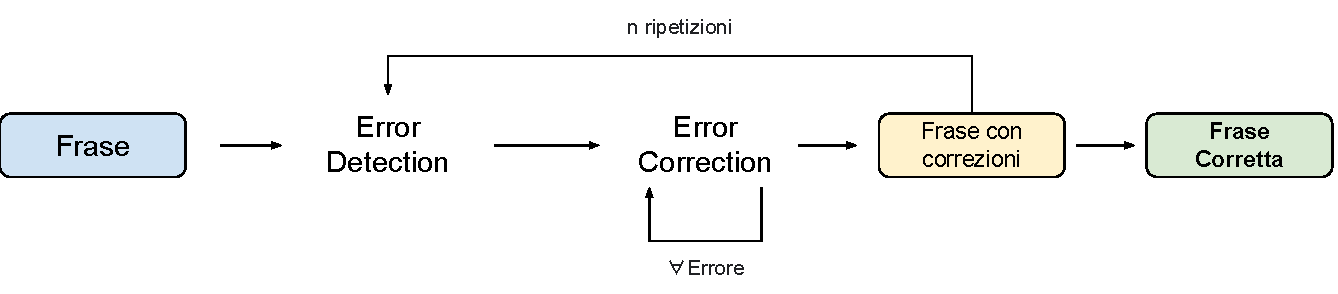
\includegraphics[width=\textwidth]{immagini/metodologia/generale}
\caption{Schema riassuntivo della Metodologia}
\label{fig:met_generale}
\end{figure}


\subsection{Error Detection}
\label{sec:met_errdet}

Lo scopo dell'error detection è quello di contrassegnare gli errori presenti all'interno della frase per la successiva fase di error correction. Dato che l'error correction corregge gli errori a livello di token, vengono contrassegnati per la fase successiva tutti i token contenenti errori. A tale scopo, è necessario in primis tokenizzare la frase di partenza. Successivamente tutti i token contenenti errori vengono marcati per la correzione.\\
Quanto appena spiegato è riportato nello schema in \autoref{fig:met_errdet}.

\begin{figure}[H]
\centering
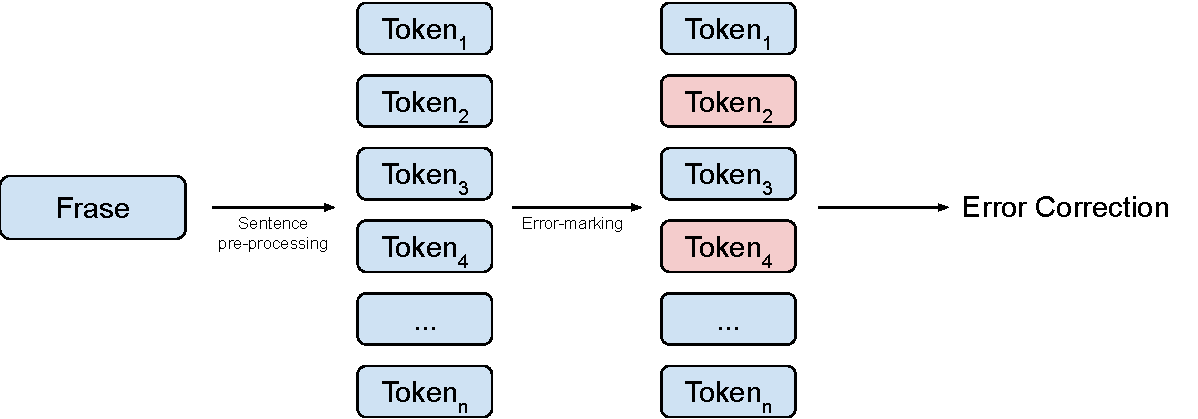
\includegraphics[width=\textwidth]{immagini/metodologia/error_detection}
\caption{Schema del processo di error detection}
\label{fig:met_errdet}
\end{figure}

\subsection{Error Correction}
\label{sec:met_errcor}

Il processo di error correction si basa sul BERT Masked Language Modeling. Data una qualsiasi frase, è possibile sostituire una parola con la stringa \textit{[MASK]}, detta maschera. Dando in input la frase mascherata al modello BERT, esso produrrà una serie di parole (da qui in poi candidati) associate alla loro probabilità di corrispondere al token mascherato.

\paragraph{Esempio} Data la frase 
\begin{center}
\textit{"che assistono ragazze in difficoltà, le persone \underline{soie} e abbandonate, gli ammalati e gli anziani."}
\end{center}
la parola \textit{"soie"} sottolineata è stata individuata come errore. \E\ quindi necessario mascherala, per dare la frase in input al modello BERT. La frase diventa dunque:
\begin{center}
\textit{"che assistono ragazze in difficoltà, le persone [MASK] e abbandonate, gli ammalati e gli anziani."}
\end{center}
BERT produce quindi una lista di candidati, di cui sono riportati solo i primi 5:
\begin{itemize}
\item \textit{"sole"} con probabilità 0.42
\item \textit{"anziane"} con probabilità 0.28
\item \textit{"povere"} con probabilità 0.08
\item \textit{"care"} con probabilità 0.03
\item \textit{"disabili"} con probabilità 0.01
\end{itemize}
\ \\
Bisogna sottolineare come la parola originale sia trasparente al modello BERT. Ciò significa che i candidati prodotti dal modello sono del tutto indipendenti dalla parola originale, e sono inferite unicamente dal contesto derivato dal resto della frase.\\
La fase di error correction inizia con i token contrassegnati come errore nella fase precedente. Si procede mascherando il primo token errato all'interno della frase. Siccome BERT necessità di una frase, e non di un'insieme di token, è necessario detokinizzare la frase. Fatto ciò è possibile produrre i candidati per la correzione, come mostrato in \autoref{fig:met_errgen}.

\begin{figure}[H]
\centering
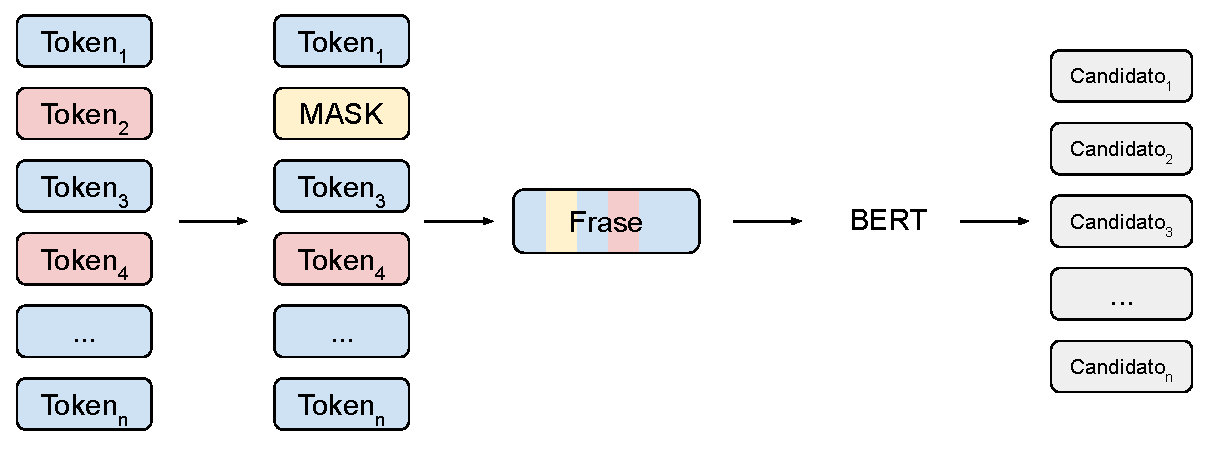
\includegraphics[width=\textwidth]{immagini/metodologia/generazione_candidati}
\caption{Schema del processo di generazione dei candidati}
\label{fig:met_errgen}
\end{figure}


Fra i vari candidati proposti da BERT ne viene scelto solamente uno, che viene determinato sulla base di alcuni criteri che tengono conto anche del token originale contente l'errore. Può però accadere che nemmeno il candidato sia la correzione adatta: si pensi al caso in cui l'error detection contrassegna un token corretto come errore, o ad una frase in cui bert non produce la parola corretta fra i candidati. Ogni candidato scelto deve quindi passare un ulteriore filtro, che ha lo scopo di distinguere queste evenienze. Nel caso il candidato non passi il filtro, il sistema ignora la correzione; in caso contrario, la correzione viene sostituita al token mascherato. Quanto appena descritto è rappresentato nello schema in \autoref{fig:met_errgen}.
\begin{figure}[H]
\centering
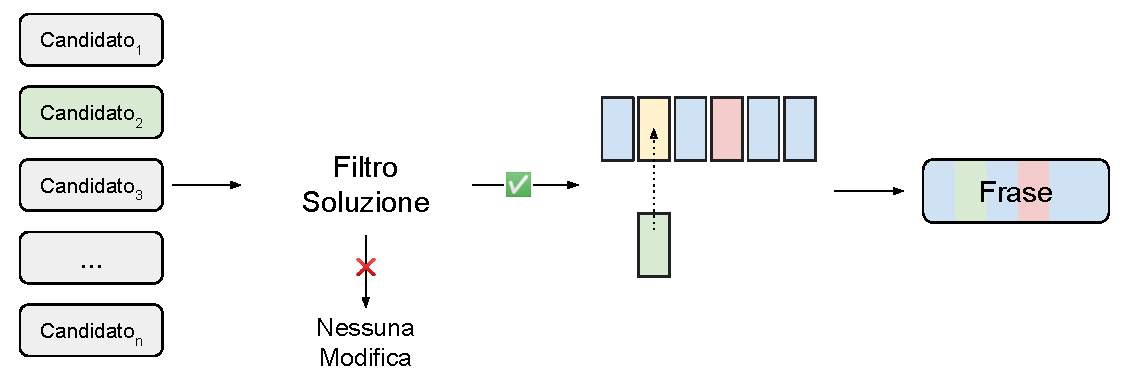
\includegraphics[width=\textwidth]{immagini/metodologia/scelta_candidati}
\caption{Schema del processo di scelta dei candidati}
\label{fig:met_errgen}
\end{figure}
Il processo appena descritto si ripete per ogni errore contrassegnato durante la fase di error detection. Una volta completata la correzione dell'ultimo token errato, la fase di error correction può dirsi conclusa.


%\begin{figure}[H]
%\centering
%\includegraphics[width=\textwidth]{immagini/metodologia}
%\caption{blabla}
%\label{fig:met_}
%\end{figure}


